%\documentclass{beamer}
\documentclass[11pt,handout,pdf,hyperref={unicode}]{beamer}
\setbeamertemplate{navigation symbols}{}

\usepackage[T2A]{fontenc}
\usepackage[utf8]{inputenc}
\usepackage[english,russian]{babel}
\usepackage[style=authoryear]{biblatex}
\usepackage{listings}
\renewcommand*{\nameyeardelim}{\addcomma\addspace}
\graphicspath{ {images/} }
\DeclareGraphicsExtensions{.png,.pdf}
\addbibresource{custom.bib}
\usetheme{Warsaw}

\addtobeamertemplate{navigation symbols}{}{%
    \usebeamerfont{footline}%
    \usebeamercolor[black]{footline}%
    \hspace{10em}%
    \insertframenumber/\inserttotalframenumber
}

\lstdefinelanguage{orgmode}
{
  % list of keywords
  morekeywords={
    TODO, DONE, LOGBOOK, END
  },
  sensitive=false, % keywords are not case-sensitive
  morecomment=[s]{/*}{*/}, % s is for start and end delimiter
  morestring=[b]" % defines that strings are enclosed in double quotes
}

\usepackage{color}
\definecolor{eclipseBlue}{RGB}{42,0.0,255}

\lstset{
  language={orgmode},
  basicstyle=\small\ttfamily, % Global Code Style
  columns=fixed, % make all characters equal width
  keepspaces=true, % does not ignore spaces to fit width, convert tabs to spaces
  showstringspaces=false, % lets spaces in strings appear as real spaces
  breaklines=true, % wrap lines if they don't fit
  frame=trbl, % draw a frame at the top, right, left and bottom of the listing
  numberstyle=\tiny\ttfamily, % style of the line numbers
  keywordstyle=\color{eclipseBlue}, % style of keywords
}

\newcommand{\backupbegin}{
   \newcounter{finalframe}
   \setcounter{finalframe}{\value{framenumber}}
}
\newcommand{\backupend}{
   \setcounter{framenumber}{\value{finalframe}}
}

%Information to be included in the title page:
\title[Тайм-трекинг на блокчейне]{Тайм-трекинг пользовательских действий на распределенной блокчейн-сети}

\begin{document}


\author[Михаил Волхов, M3438]{
  Студент: Михаил Волхов, M3438\\
  Руководитель: Штукенберг Д.Г., тьютор кафедры КТ \\
  Рецензент: Чепурной А.И, специалист, IOHK Research
}
\institute{Кафедра Компьютерных Технологий \\ факультет Информационных Технологий и Программирования \\ Университет ИТМО, Санкт-Петербург}
\date{16 мая 2017}

\frame{\titlepage}

\section{Введение и цели}

\subsection{Используемые технологии}

\begin{frame}
  \frametitle{Криптовалюта}

  Платежная система, основанная на блокчейне.
  \begin{itemize}
  \item Широкая функциональность:
  \begin{itemize}
    \item Скриптинг/смарт-контракты: скрипт сам решает как
      снимать с себя деньги.
    \item HD-кошельки.
    \item Multisig транзакции.
  \end{itemize}
  \item Глобальная история, публичность, распределённость.
  \end{itemize}
\end{frame}

\begin{frame}[fragile]
  \frametitle{Тайм-трекинг}

  Ассоциирует активности пользователя с набором временных интервалов
  (сколько времени потрачено на задачу $X$).

  \begin{itemize}
  \item Зачем: анализ данных, составление статистики и отчетностей.
  \item Примеры: toggl, arbtt, youtrack, org-mode, strava.
  \end{itemize}

  Недостающая функциональность:
  \begin{itemize}
  \item Автоматизированный сбор и анализ статистики.
  \item Мультипользовательские (совместные) активности.
  \end{itemize}

\end{frame}

\begin{frame}
  \frametitle{Общая идея}

  Эти задачи тайм-трекинга блокчейн решает прямолинейно:
  \begin{itemize}
  \item Мультипользовательских активности -- транзакции криптовалюты.
    \begin{itemize}
    \item Доказательство совместной деятельности это подписи транзакции.
    \end{itemize}
  \item Сбор статистики с помощью смарт-контракта: оценка
    пользователей и распределение рейтинга.
  \item Свойства рейтинга за счет использования блокчейна:
    \begin{itemize}
    \item Псевдопубличность: открытый доступ к данным, зная адреса
      пользователей.
    \item Финальность: невозможность скорректировать.
    \end{itemize}
  \end{itemize}
\end{frame}

\subsection{Поставленная задача}

\begin{frame}
  \frametitle{Задача и примеры} Задача: разработать модификацию
  криптовалюты:
  \begin{itemize}
  \item Имеет функциональность тайм-трекинга.
  \item Мультипользовательские транзакции и контракты, выставление рейтинга.
  \item Не нарушает гарантий криптовалюты.
  \end{itemize}

  Примеры использования:
  \begin{itemize}
    \item Оптимизация отношений внутри (рабочего) коллектива,
      формальные обязанности и доказательства их (не)выполнения.
    \item Трекинг занятий спортом, контракт как норма тренировок.
  \end{itemize}
\end{frame}

\section{Проделанная работа}

\subsection{Общий обзор работы}

\begin{frame}
  \frametitle{Схема алгоритма}
  \begin{figure}[t]
  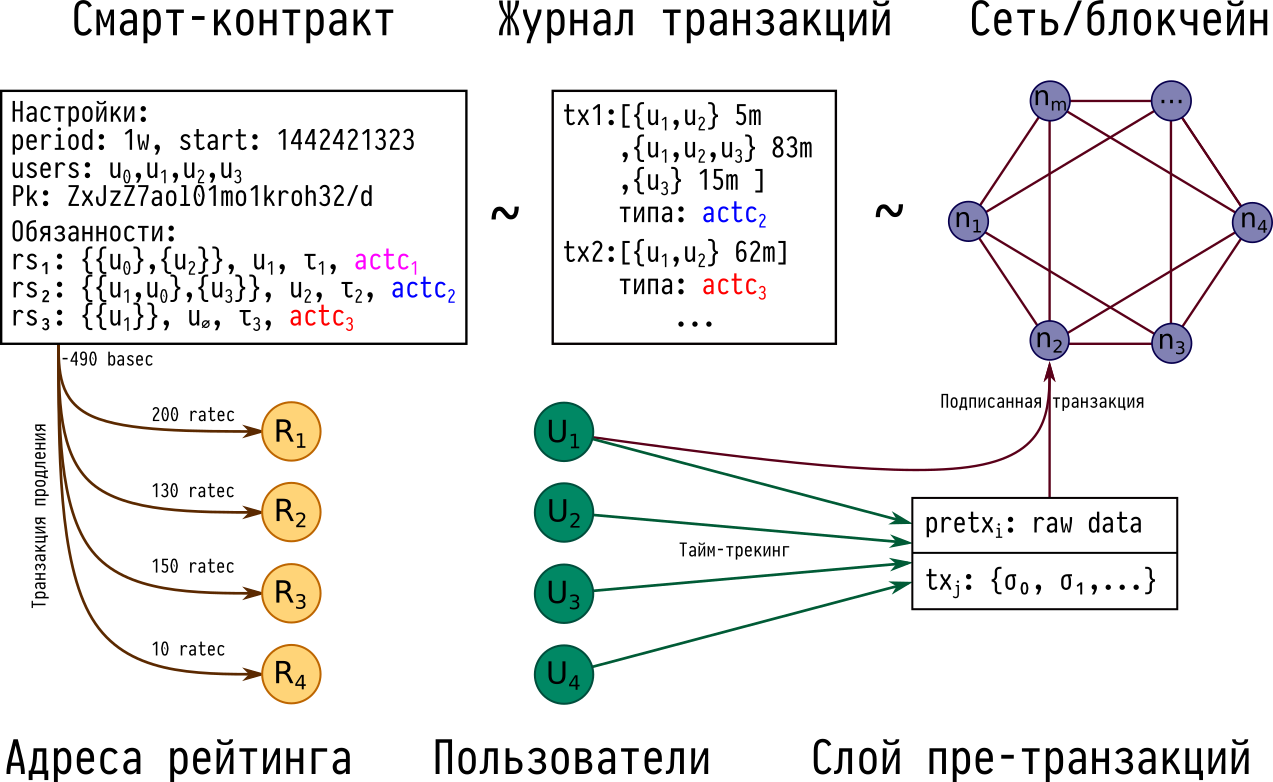
\includegraphics{presentation_big_scheme}
  \centering
  \end{figure}

\end{frame}

\begin{frame}
  \frametitle{Структура работы}

  \begin{enumerate}
  \item Интеграция цветных монет в Ouroboros \parencite{ouroboros}:
    представляют типы активностей и рейтинг.
  \item Спроектирована структура:
    \begin{itemize}
    \item Мультипользовательских активностей,
    \item Обязанностей (контракта),
    \item Функция распределения рейтинга (доказаны свойства).
    \end{itemize}
  \item Интеграция этих компонент в транзакции и скрипты криптовалюты.
  \item Проанализирована проблема сбора подписей, свойства
    приведенного алгоритма.
  \end{enumerate}

\end{frame}

\subsection{Подробное описание компонент}

\begin{frame}
  \frametitle{Цветные монеты}

  Надстройка над криптовалютой, добавляющее к монете тег цвета
  \parencite{epobc} \parencite{oap}.

  \begin{itemize}
  \item Реализация в работе предусматривает покраску монет внутри
    транзакции в другой цвет.
  \item Это усложняет валидацию транзакции.
  \item Показано, как сводить задачу валидации к задаче о полном
    потоке в графе.
  \end{itemize}
\end{frame}

\begin{frame}
  \frametitle{Обязательства}

  Контракт -- множество обязательств вида $(supp, rec, \tau,
  actc_i)$:
  \begin{itemize}
  \item Множество поставщиков $supp$.
  \item Получатель $rec$.
  \item $\tau$ -- сколько нужно уделить времени в период контракта.
  \item Тип активности $actc_i$.
  \end{itemize}
\end{frame}

\begin{frame}
  \frametitle{Транзакции}

  Эмуляция тайм-трекинга с помощью транзакций криптовалюты.
  \begin{itemize}
  \item Пре-транзакция: для каждого пользователя $u_i$ интервалы $u_i
    \sim [\tau_{start}, \tau_{end}]$.
  \item Конвертация в транзакцию с сохранением интервалов.
  \item Перевод монет цвета $actc_i$ на специальные адреса
    активностей.
  \end{itemize}
\end{frame}

\begin{frame}
  \frametitle{Выставление рейтинга}

  Функция выставления рейтинга пользователя $r_f : U \rightarrow \mathbb{N}$:
  \begin{itemize}
  \item $r_f(u) \in [0,p_m]$, где $p_m \sim$ обязательствам $u$.
  \item $r_f(u) = p_m$, если все обязательства $u$
    удовлетворены. $r_f(u) = 0$, если ни одно.
  \item $r_f \sim$ важности $u$ в каждом обязательства $rs$
    ($supp$ как коалиционная игра).
  \item $r_f(u) \sim$ времени потраченного пользователем $u$ на
    удовлетворение $rs$.
  \end{itemize}

\end{frame}

\begin{frame}
  \frametitle{Смарт-контракт}

  Распределение рейтинга производится с помощью транзакции продления $Tx$:
  \begin{itemize}
  \item $Tx$ конвертирует средства на счету контракта в монеты рейтинга.
%  \item Монеты трекинга активностей $actc$ переиспользуются.
  \item Деньги со скрипта могут быть сняты только если:
  \begin{itemize}
    \item Рейтинговые адреса совпадают с таковыми в контракте.
    \item Указанное распределение рейтинга в $Tx$ верно.
  \end{itemize}
  \item Может быть выполнена любым участником контракта.
  \end{itemize}
\end{frame}

\subsection{Дополнения и выводы}

\begin{frame}
  \frametitle{Дополнения}

  \begin{itemize}
  \item Слой формирования транзакций и сбора подписей:
      \begin{itemize}
      \item Описан API сервиса.
      \item Рассмотрена централизованная и децентрализованная модель;
        предложено решение с Kademlia DHT спроектированное под
        Ouroboros.
      \end{itemize}
  \item Возможность интеграции реальных денежных штрафов.
  \item Неполное доверие, рецензенты обязанностей.
  \item Обзор свойств рейтинга, приватность данных.
  \end{itemize}
\end{frame}

\begin{frame}
  \frametitle{Результаты}

  Решение для тайм-трекинга поверх Ouroboros:
  \begin{itemize}
  \item Интеграция цветных монет: анализ, реальная схема.
  \item Обязанности, контракт, транзакции, функция распределения
    рейтинга.
  \item Интеграция вышеперечисленного с криптовалютой.
  \item Слой пре-транзакций, дополнения и анализ.
  \end{itemize}
   \begin{center}
    \Huge Спасибо за внимание!
  \end{center}
\end{frame}

\backupbegin
\section{}

\begin{frame}
  \frametitle{Актуальность: блокчейн}

  \begin{itemize}
  \item Совместные активности с подписями.
  \item Интеграция денежных штрафов.
  \item Автоматическая плата за использование сервиса.
  \item Универсальность: сервисов много, рейтинг -- один, глобальный.
  \item Надежность: рейтинг финальнен и независим от политики
    подсервисов.
  \end{itemize}
\end{frame}

\begin{frame}
  \frametitle{Актуальность: цветные монеты}

  В представленном решении:
  \begin{itemize}
  \item Модификация популярного готового решения (EPOBC, OAP, Colu).
  \item Мнемонически просто и эффективно, по сравнению с другими
    способами кодирования информации о типе активности.
  \end{itemize}

  В общем смысле:
  \begin{itemize}
  \item Эмуляция других ресурсов и типов валют (золото, нефть, акции).
  \item Отслеживание движения средств без необходимости парсинга всего
    блокчейна.
  \end{itemize}
\end{frame}

\begin{frame}
  \frametitle{Валидация цветной транзакции 1/2}

  Добавляем к монете тег цвета. Цвета конвертируются согласно графу
  конвертации $G_c$. Теперь валидация транзакции сложнее, чем
  проверить $\sum{in_i} \geq \sum {out_j}$.

  \begin{figure}[t]
  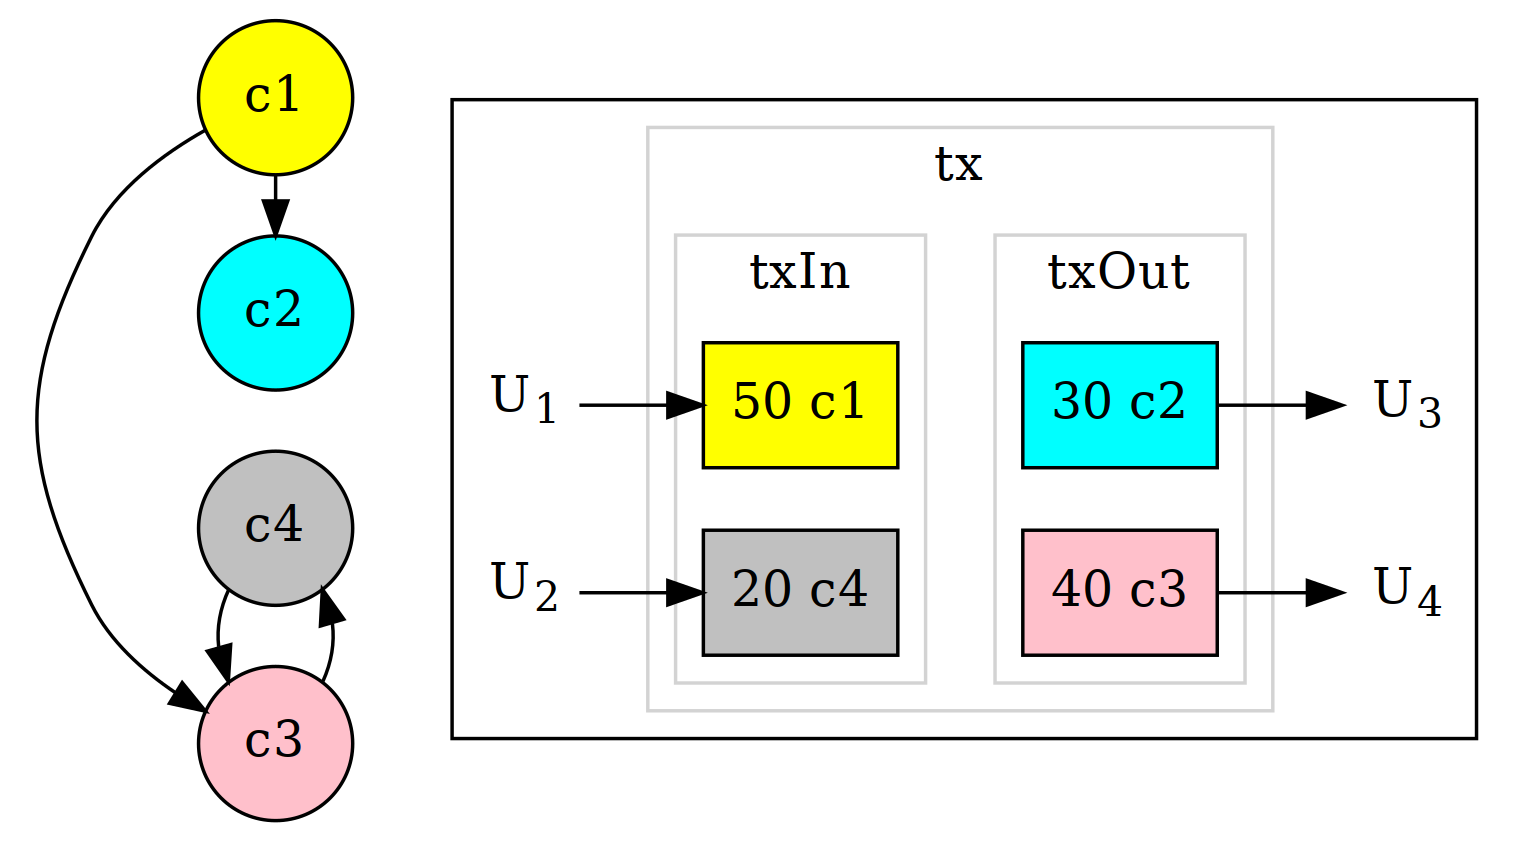
\includegraphics[scale=0.17]{pres_colortx.png}
  \centering
  \end{figure}

\end{frame}

\begin{frame}
  \frametitle{Валидация цветной транзакции 2/2}

  Хотим разбиение входов, равное выходам с точностью до покраски.

  \begin{align*}
    \exists H = \ &\bigsqcup_{i=1}^s{H_i}. \ MergeC(H) = txIn_m \ \wedge \nonumber \\
                  &\forall (n_{out},c_{out}) \in txOut . \ \exists i . \ H_i = (n_{out},c_{in}) \wedge c_{in}c_{out} \in G_c \label{eq:1}
  \end{align*}

  Сведение к задаче о максимальном потоке в графе:
  %Сведение к задаче о максимальном потоке в графе $D$, построенном из
  %$G_c$ и $Tx$.

  \begin{figure}[t]
  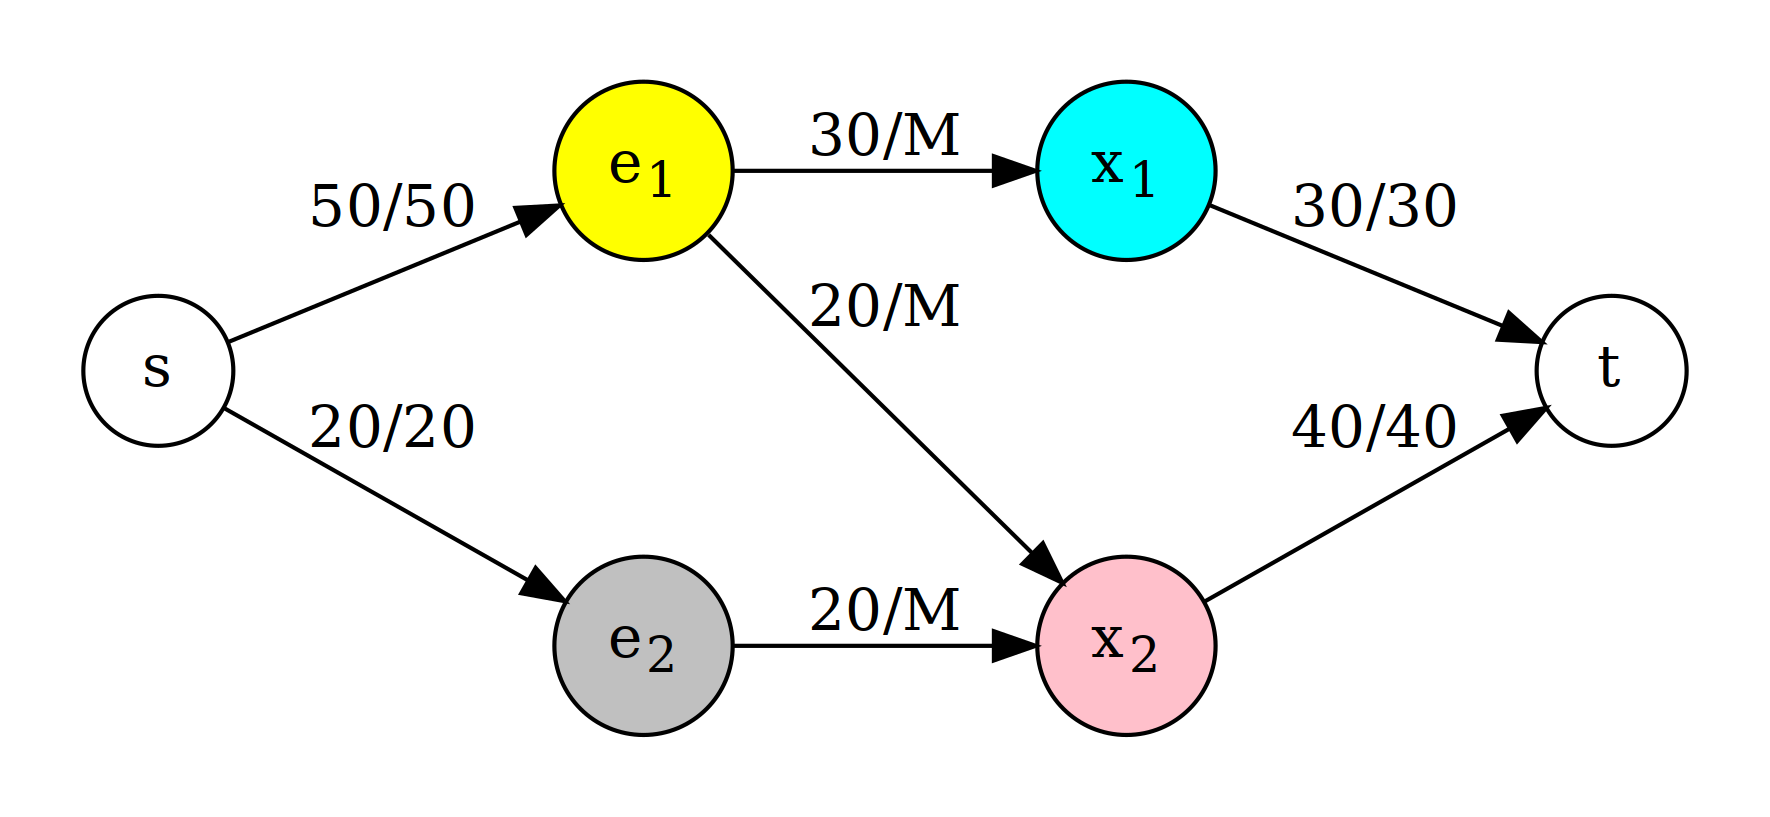
\includegraphics[scale=0.12]{pres_colortx_graph}
  \centering
  \end{figure}
\end{frame}


\begin{frame}
  \frametitle{Примеры}

  \begin{itemize}
    \item Спорт. Трекинг (совместных) тренировок, лекций. Получаем
      социальную сеть, где можно сравнивать свои спортивные достижения
      (e.g. strava).
    \item Трекинг эффорт-ориентированных задания (например,
      репетиторство). Получаем децентрализованный youdo.
    \item Отношения: трекинг обязанностей, отдыха. Получаем социальную
      сеть, где рейтинг $\sim$ эффорт партнера.
    \item Небольшая IT-компания. Трекинг митингов и рабочего время (по
      проектам). Получаем статистику для менеджеров и рейтинг
      продуктивности сотрудников (зеленые квадратики на github).
    \item Совмещение всех функциональностей в одном сервисе.
  \end{itemize}
\end{frame}

\begin{frame}
  \frametitle{Нетривиальность}

  \begin{itemize}
  \item Включает большое количество технологий (изучал zksnark'и,
    кодовую базу bitcoin).
  \item Работа в сфере криптовалют:
    \begin{itemize}
    \item Знание кодовой базы CSL/Ouroboros.
    \item Консультировался с создателями Ouroboros,
      Plutus\parencite{plutus}, разработчиками ZCash
      \parencite{zerocash}.
    \item Реализовал поддержку цветных монет в RSCoin
      \parencite{rscoin}.
    \end{itemize}
  \item Нетривиальные решения:
    \begin{itemize}
    \item HD ключи для адресов активностей.
    \item Поддержка интервальной модели в транзакциях.
    \end{itemize}
  \end{itemize}
\end{frame}

\begin{frame}
  \frametitle{Пользовательские отношения, цели}

  Модель доверия:
  \begin{itemize}
  \item По умолчанию -- полное доверие внутри контракта.
  \item Дополнение: ревьюеры обязанности, позволяют решить проблему с
    неполным доверием.
  \end{itemize}

  Какие задачи решаются наиболее эффективно?
  \begin{itemize}
  \item Измерение эффорта, а не результата работы.
    \begin{itemize}
    \item Software development effort estimation -- можно мерить только время.
    \end{itemize}
  \item Ориентированность на длительные контракты, не на конкретные задачи.
  \end{itemize}

\end{frame}

\backupend

\end{document}
